\documentclass{beamer}
\usepackage[utf8]{inputenc}
\usepackage[UKenglish]{babel}
\usepackage[UKenglish]{isodate}
\usepackage{amsmath}
\usepackage{mathtools}
\usepackage{tikz}
\usepackage{complexity}
\usepackage[style=authoryear]{biblatex}

\usetikzlibrary{shapes}
\usetikzlibrary{positioning}
\usetikzlibrary{overlay-beamer-styles}
\usetikzlibrary{shapes.callouts}
\usetikzlibrary{cd}
\usetikzlibrary{calc}

\beamertemplatenavigationsymbolsempty
\usetheme{metropolis}
\setbeamercolor{background canvas}{bg=white}
\addbibresource{talk.bib}
%\usecolortheme{rose}

\definecolor{color1}{HTML}{1B9E77}
\definecolor{color2}{HTML}{D95F02}
\definecolor{color3}{HTML}{7570b3}
\definecolor{color4}{HTML}{e7298a}

\newcommand{\x}{\textcolor{color1}{x}}
\newcommand{\y}{\textcolor{color3}{y}}
\newcommand{\pP}{\textcolor{color3}{P}}
\newcommand{\dDelta}{\textcolor{color2}{\Delta}}

\newcommand{\WMC}{\textup{WMC}}
\newcommand{\WFOMC}{\textup{(W)FOMC}}
\newcommand{\WMI}{\textup{WMI}}
\newcommand{\WFOMI}{\textup{WFOMI}}
\newcommand{\AMC}{\textup{AMC}}
\newcommand{\pbp}{\textup{PBP}}
\newcommand{\SPPP}{\textup{SP}}

% 15 min introduction
% 20-25 min presentation
% 5-10 min summary
% 20-25 slides
% before it was 15 slides and 20 min
% make sure there's a clear and coherent storyline
% TODO: use \alert instead of \structure
% TODO: add a very clear example of what a model is
% TODO: could add the step-by-step walkthrough of what FOKC looks like
% TODO: add a slide about other approaches to WFOMC, making it crystal clear what my contributions are

\author{\textbf{Paulius Dilkas} \inst{1} \and Vaishak Belle \inst{2}}
\title{Recursive Solutions to \\First-Order Model Counting}
\institute{\inst{1} National University of Singapore, Singapore \and \inst{2} University of Edinburgh, UK}
\date{TODO: date}

\begin{document}
\addtobeamertemplate{block begin}{\setlength\abovedisplayskip{0pt}}

\begin{frame}[noframenumbering,plain]
  \tikz[remember picture,overlay]{
    \node at ([yshift=20pt,xshift=-20pt]current page.south)
    {
\includegraphics[height=40pt]{nus.jpg}};
    \node at ([yshift=25pt,xshift=30pt]current page.south)
    {
\includegraphics[height=40pt]{inf.png}};
    \node at ([yshift=25pt,xshift=75pt]current page.south)
    {
\includegraphics[height=40pt]{ecr.jpg}};
    \node at ([yshift=20pt,xshift=140pt]current page.south)
    {
\includegraphics[height=20pt]{epsrc.png}};
  }
  \titlepage
\end{frame}

\begin{frame}{What Computers Can and Cannot Do}
  \begin{tikzpicture}[remember picture,overlay]
    \node[right=0.7cm] at (current page.west) (stickman) {
\includegraphics[height=0.5\textheight]{stickman.png}};
    \node<-4>[left,shift=({0, -2})] at (current page.east) (computer) {
\includegraphics[height=0.5\textheight]{happy_computer}};
    \node<2>[ellipse callout, draw, right=0cm, callout relative pointer={(-1, -0.5)}] at (stickman.north east) {$\int_{-\infty}^{\infty} e^{-t^{2}}\,\mathrm{d}t$};
    \node<2>[ellipse callout, draw, left=-0.5cm, below=0.5cm] at (computer.north west) {$\sqrt{\pi}$};
    \node<3>[ellipse callout, draw, right=-1cm, callout relative pointer={(-2.5, -0.5)}] at (stickman.north east) {Produce a schedule for the nurses at NUH.};
    \node<3>[ellipse callout, draw, below=0.5cm, shift=({-0.5,0}), callout relative pointer={(0.5, -0.25)}] at (computer.north west) {
\includegraphics[width=0.1\textwidth]{schedule}};
    \node<4>[ellipse callout, draw, right=0cm, callout relative pointer={(-1, -0.15)}] at (stickman.north east) {Describe this picture. 
\includegraphics[width=0.25\textwidth]{cat.jpg}};
    \node<4>[ellipse callout, draw, below=0.5cm, shift=({-0.5,0.5}), callout relative pointer={(0.5, -0.5)}] at (computer.north west) {It's a cat with its eyes closed.};
    \node<5>[ellipse callout, draw, right=0cm, callout relative pointer={(-1, -0.15)}, text width=5cm] at (stickman.north east) {If I shuffle a deck of \alert{$n$} cards, how many possible outcomes are there?};
    \node<5>[left,shift=({-1, -1})] at (current page.east) (computer2) {
\includegraphics[height=0.5\textheight]{overheating_computer}};
    \node[shift=({1.3, 0.1})] at (current page.south west) {\tiny \color{lightgray}{Vector art by Vecteezy.com}};
  \end{tikzpicture}
\end{frame}

\begin{frame}{Who Cares About Counting?}
  \begin{columns}
    \begin{column}{0.5\textwidth}
      \pause
      \begin{block}{\alert{Probabilistic Programming}}
        \centering
        
\includegraphics[width=\textwidth]{programming.png}
      \end{block}
      \pause
      \begin{block}{\alert{Neuro-symbolic AI}}
        \centering
        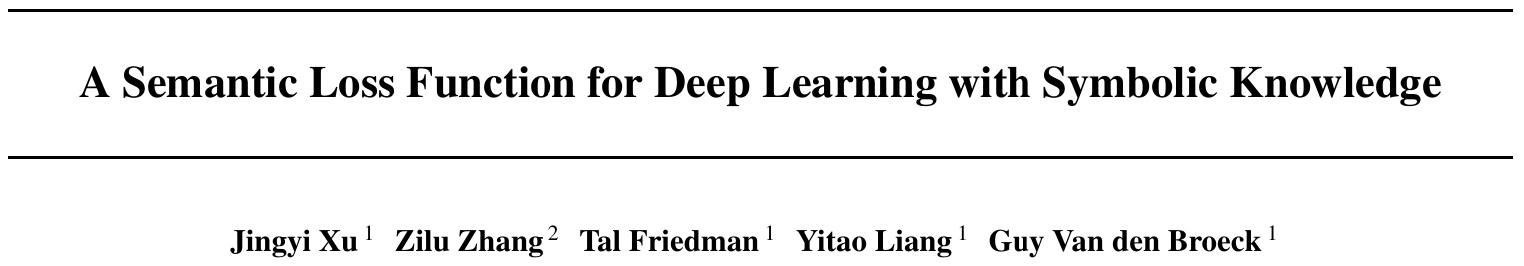
\includegraphics[width=\textwidth]{neurosymbolic.png}
      \end{block}
      \pause
      \begin{block}{\alert{Natural Language Processing}}
        \centering
        
\includegraphics[width=\textwidth]{knowledge.png}
      \end{block}
      \pause
    \end{column}
    \begin{column}{0.5\textwidth}
      \begin{block}{\alert{Robotics}}
        \centering
        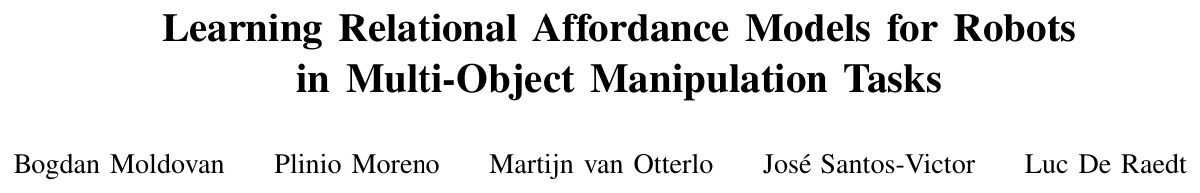
\includegraphics[width=\textwidth]{ICRA.png}
      \end{block}
      \pause
      \begin{block}{\alert{Bioinformatics}}
        \centering
        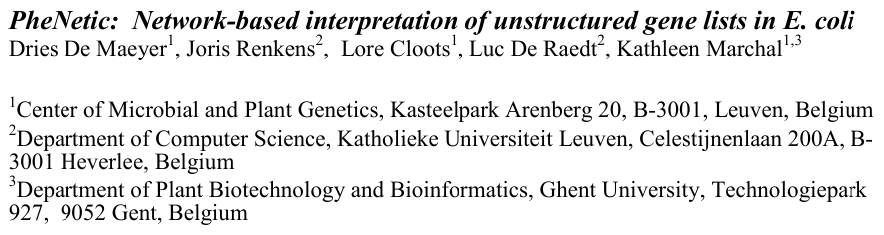
\includegraphics[width=\textwidth]{bio.png}
      \end{block}
      \pause
      \begin{block}{\alert{Combinatorics}}
        \centering
        
\includegraphics[width=\textwidth]{recurrence.png}
      \end{block}
    \end{column}
  \end{columns}
\end{frame}

\begin{frame}[fragile]{(Some of the) Many Ways to Count}
  \begin{center}
    \begin{tikzcd}[remember picture]
      |[alias=WMI,visible on=<7->]|\WMI{} & |[visible on=<7->]|\WFOMI{} \\
      |[alias=WMC]|\#\SAT{}/\WMC{} \arrow[u,visible on=<7->] \ar[d,visible on=<8->] \ar[r,visible on=<5->] & |[visible on=<5->]|\WFOMC{} \arrow[u,visible on=<7->] \ar[d,visible on=<8->] \\
      |[alias=PBP,visible on=<8->]|\AMC{}, \pbp{} & |[alias=SP,visible on=<8->]|\SPPP{}
    \end{tikzcd}
  \end{center}
  \begin{tikzpicture}[overlay,remember picture]
    \begin{scope}[transform canvas={xshift=-3em}]
      \draw[->,draw=gray] ($(WMC)+(0,0.1)$)--($(WMI)+(0,0.5)$) node[midway,left,visible on=<7->] {\color{gray}{$\sum \to \int$}};
      \draw[->,draw=gray] ($(WMC)-(0,0.1)$)--($(PBP)-(0,0.5)$) node[midway,left,visible on=<8->] {\color{gray}{Generalising weights}};
    \end{scope}
    \begin{scope}[transform canvas={yshift=-2em}]
      \draw[->,draw=gray] ($(PBP)-(1,0)$)--($(SP)+(1,0)$) node[midway,below,visible on=<5->] {\color{gray}{From propositional to first-order logic}};
    \end{scope}
  \end{tikzpicture}
  \vfill
    \begin{overprint}
      \onslide<1,2>
      \begin{block}{\#SAT~\color{gray}{\parencite{DBLP:journals/tcs/Valiant79}}}
        \begin{itemize}
          \item Input formula: $\x \lor \y$
          \item Interpretations: $\emptyset$, $\{\, \x \,\}$, $\{\, \y \,\}$,
                $\{\, \x, \y \,\}$
          \item Models: $\{\, \x \,\}$, $\{\, \y \,\}$, $\{\, \x, \y \,\}$
          \item<2-> Answer (model count): 3
        \end{itemize}
      \end{block}
      \onslide<3,4>
      \begin{block}{Weighted Model Counting~\color{gray}{\parencite{DBLP:journals/ai/ChaviraD08}}}
        \begin{itemize}
          \item Input formula: $\x \lor \y$
          \item Input weights: $\begin{aligned}[t]
                                  &w(\x) = 0.3\text{, }w(\neg \x) = 0.7,\\
                                  &w(\y) = 0.2\text{, }w(\neg \y) = 0.8
                                \end{aligned}$
          \item<4-> Answer (weighted model count):
                $w(\x)w(\y) + w(\x)w(\neg \y) + w(\neg \x)w(\y) = 0.44$
        \end{itemize}
      \end{block}
      \onslide<5,6>
      \begin{block}{(Weighted) (Symmetric) First-Order Model Counting\\
          \color{gray}{\parencite{DBLP:conf/ijcai/BroeckTMDR11}}}
        \begin{itemize}
          \item Input formula: $\forall \x \in \Delta\text{. }\pP(\x)$
          \item Input weights: $w^{+}(\pP) = 0.3$, $w^{-}(\pP) = 0.7$
          \item Input domain size(s): $|\dDelta| = 2$
          \item<6-> Answer: ${(w^{+}(\pP))}^{|\dDelta|} = 0.09$
        \end{itemize}
      \end{block}
      \onslide<7>
      \begin{block}{Extensions to Continuous Domains}
        \begin{itemize}
          \item Weighted model integration
          \begin{itemize}
            \item \color{gray}{\parencite{DBLP:conf/ijcai/BellePB15}}
          \end{itemize}
          \item Weighted first-order model integration
          \begin{itemize}
            \item \color{gray}{\parencite{DBLP:conf/uai/FeldsteinB21}}
          \end{itemize}
        \end{itemize}
      \end{block}
      \onslide<8>
      \begin{block}{Generalisations of the weight function}
        \begin{itemize}
          \item Algebraic model counting
          \begin{itemize}
            \item \textcolor{gray}{\parencite{DBLP:journals/japll/KimmigBR17}}
            \item From $\mathbb{R}_{\ge 0}$ to commutative semirings
          \end{itemize}
          \item Pseudo-Boolean projection~\textcolor{gray}{\parencite{DBLP:conf/sat/DilkasB21}}
          \begin{itemize}
            \item Weights not necessarily on literals
          \end{itemize}
          \item Semiring programming~\color{gray}{\parencite{DBLP:journals/ijar/BelleR20}}
        \end{itemize}
      \end{block}
    \end{overprint}
\end{frame}
% maybe mention #CSP and other non-SAT ways of counting (SMT?, counting paths in automata and directed graphs)

% TODO: for future work, come back to this slide and add more arrows (e.g., beyond FOL)

% TODO: a big chunk of the introduction should provide motivation to my work

\begin{frame}{Some Elementary Counting}
  \begin{exampleblock}{A Counting Problem}
    Suppose this room has \alert{$n$} seats, and there are \alert{$m \le n$}
    people in the audience. How many ways are there to seat everyone?
  \end{exampleblock}

  \pause
  More explicitly, we assume that:
  \begin{itemize}
  \item each attendee gets exactly one seat,
  \item and a seat can accommodate at most one person.
  \end{itemize}

  \pause
  \alert{Answer:} $n^{\underline{m}} = n \cdot (n-1)\cdots(n-m+1)$.

  Note: this problem is equivalent to counting \alert{$[m] \to [n]$} injections.

\end{frame}
% wouldn't it be nice if we could just describe this problem and have an algorithm solve it for us?

\begin{frame}{Let's Express This Problem in Logic!}
  \begin{itemize}
    \item Let \alert{$\Gamma$} and \alert{$\Delta$} be sets (i.e., domains)
    \begin{itemize}
      \item such that \alert{$|\Gamma| = m$}, and \alert{$|\Delta| = n$}.
    \end{itemize}
    \item Let \alert{$P \subseteq \Gamma \times \Delta$} be a relation (i.e.,
          predicate) over \alert{$\Gamma$} and \alert{$\Delta$}.
    \item We can describe all of the constraints in first-order logic:
    \begin{itemize}
      \item \pause each attendee gets a seat (i.e., at least one seat)
      \[
        \forall x \in \Gamma\text{. }\exists y \in \Delta\text{. }P(x, y)
      \]
      \item \pause one person cannot occupy multiple seats
      \[
        \forall x \in \Gamma\text{. }\forall y, z \in \Delta\text{. }P(x, y) \land P(x, z) \Rightarrow y=z
      \]
      \item \pause one seat cannot accommodate multiple attendees
      \[
        \forall w, x \in \Gamma\text{. }\forall y \in \Delta\text{. }P(w, y) \land P(x, y) \Rightarrow w=x
      \]
    \end{itemize}
  \end{itemize}
  \pause The first two sentences constrain \alert{$P$} to be a function, and the
  last one makes it injective.
\end{frame}
% one could also add probabilities to these sentences to say that, e.g., there is a 1% probability of somebody taking up two seats, somebody sitting on somebody else's lap, somebody sitting on the floor, etc.

\begin{frame}{Overview of the Problem}
  \begin{itemize}
    \item \alert{First-order model counting} (FOMC) is the problem of counting
          the models of a sentence in first-order logic.
    \item The \alert{(symmetric) weighted} variation of the problem adds weights
          (e.g., probabilities) to predicates.
          \begin{itemize}
            \item It is used for efficient \alert{probabilistic inference} in
                  relational models such as Markov logic networks.
          \end{itemize}
    \item None of the (implemented) (W)FOMC algorithms are able to count, e.g.,
          \alert{injective} and \alert{bijective} functions.
  \end{itemize}
  \begin{block}{Claim}
    This shortcoming can be addressed via support for \alert{recursive functions}.
  \end{block}
\end{frame}

{
  \usebackgroundtemplate{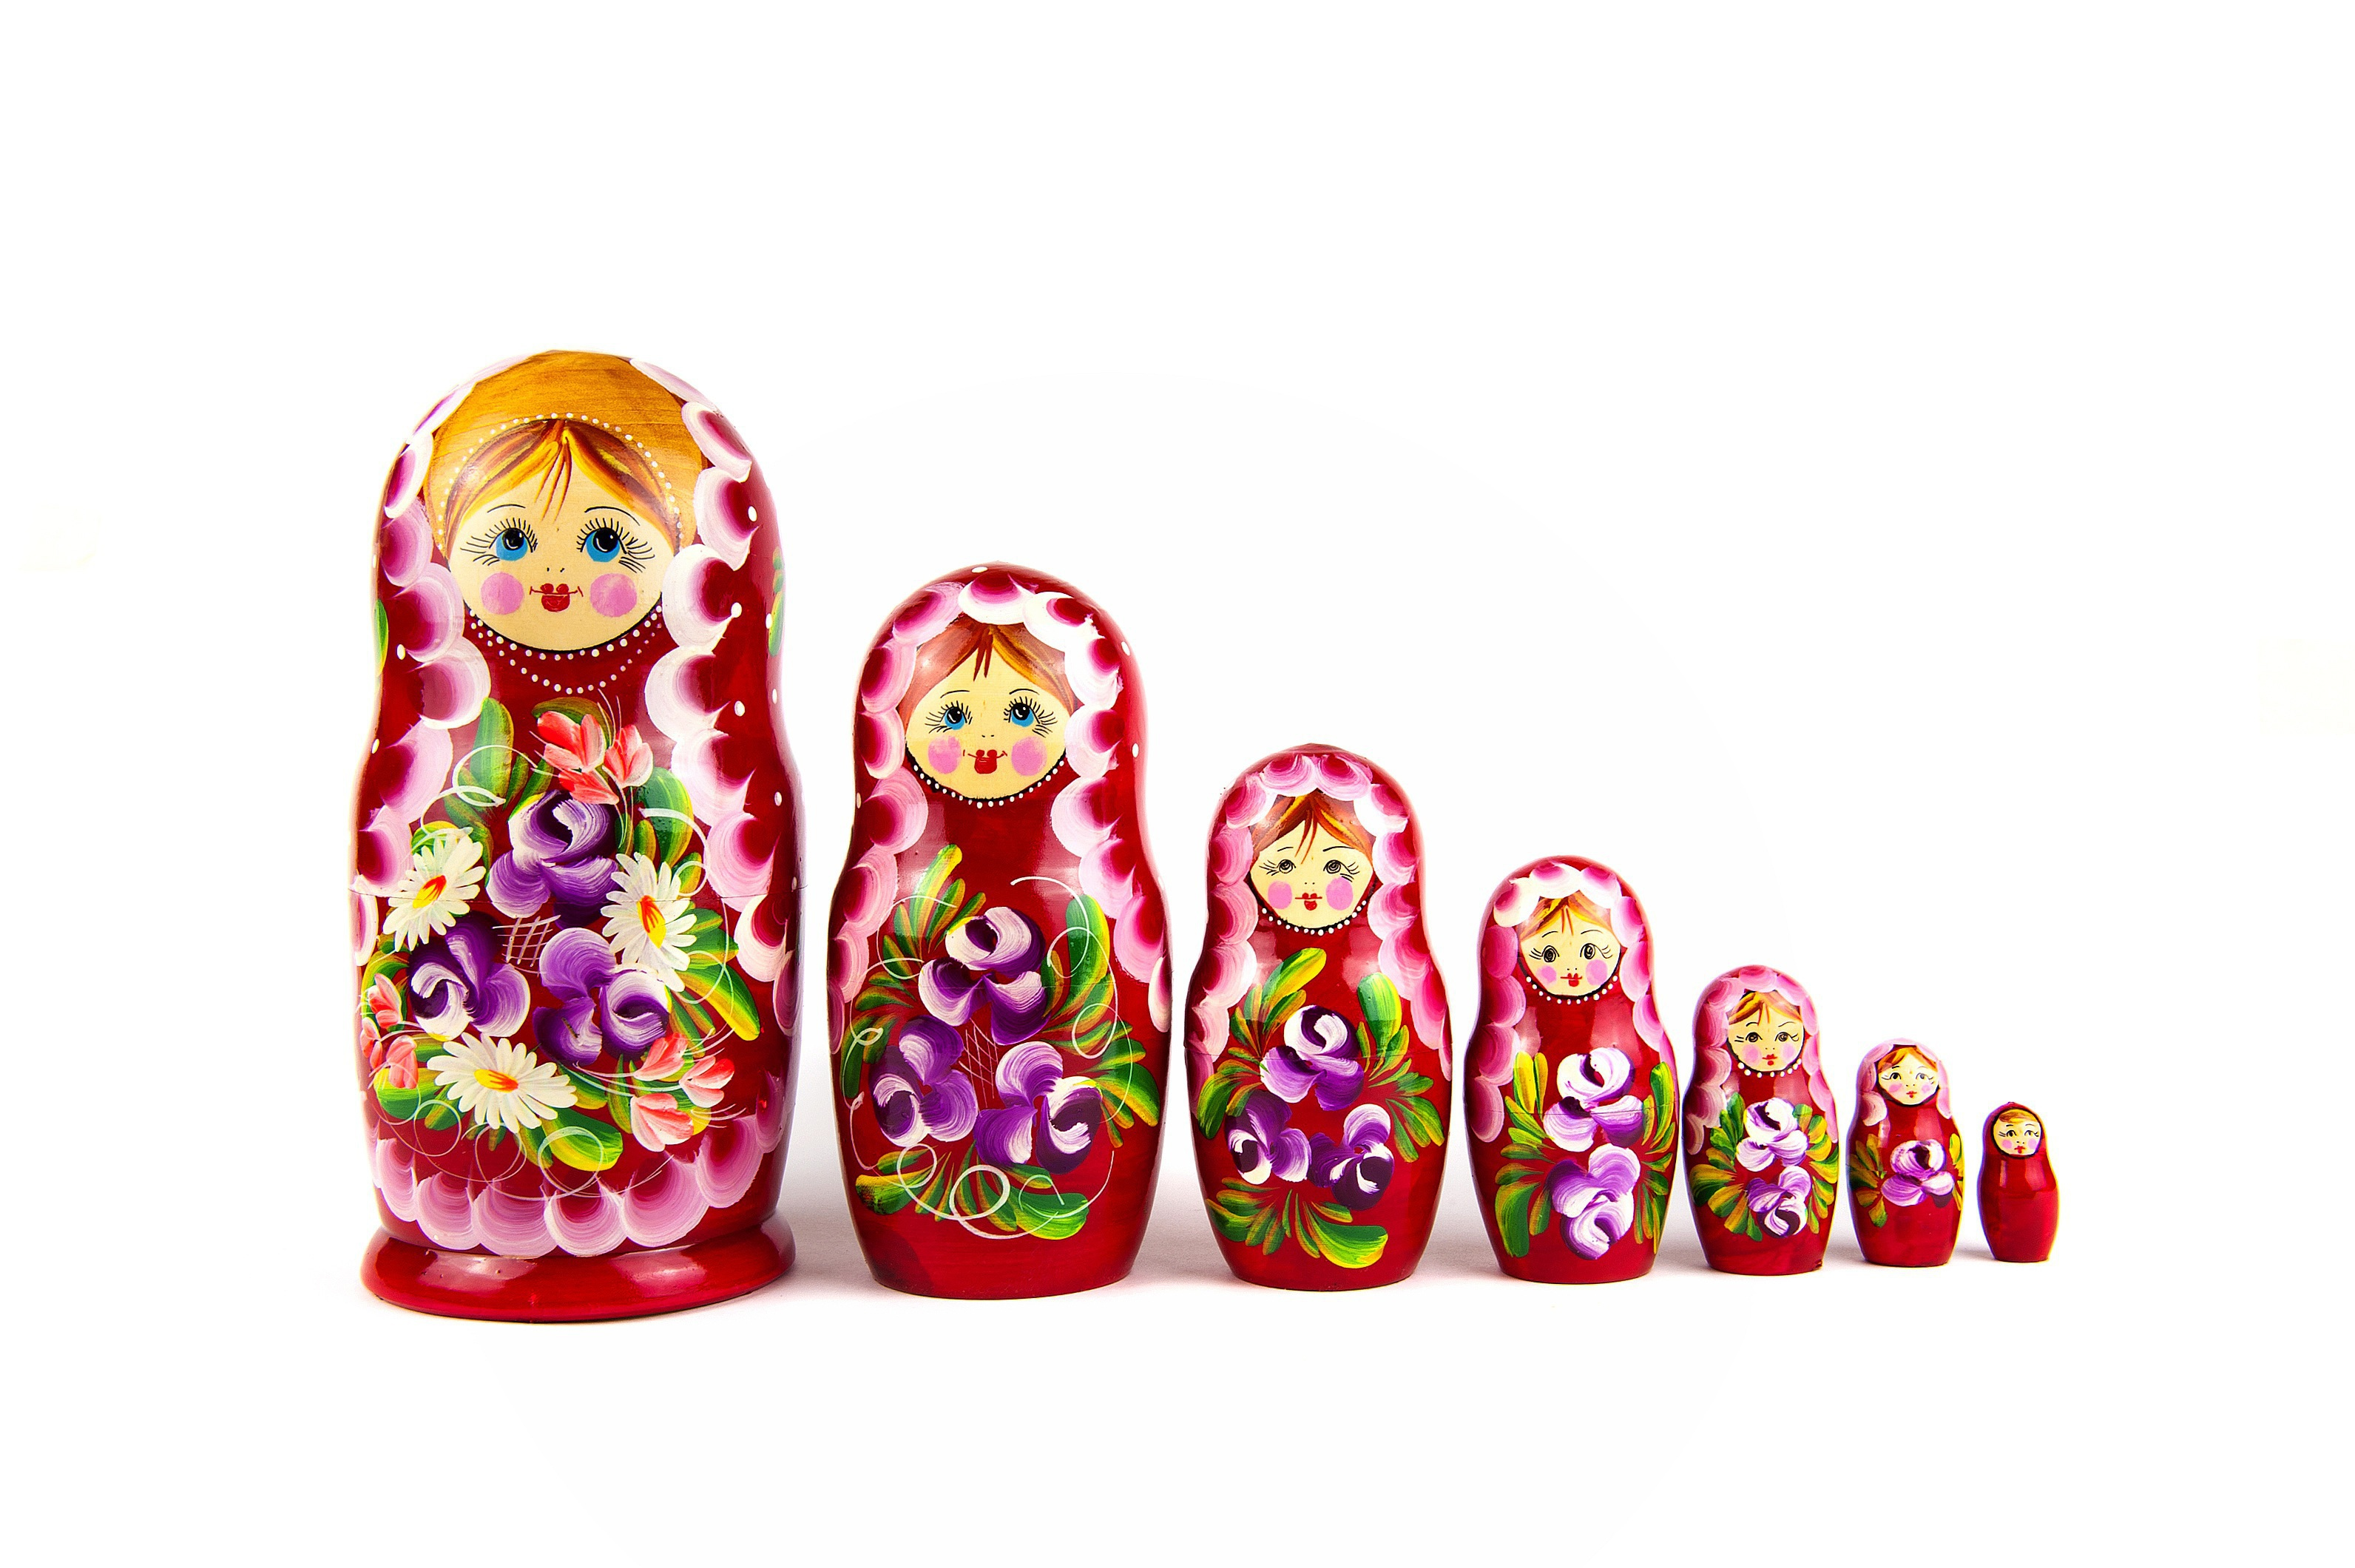
\includegraphics[keepaspectratio,width=\paperwidth]{matryoshka.jpg}}
  \begin{frame}{Recursion}
  \end{frame}
}

\begin{frame}{Back to Our Example}
  For instance, the following function counts injections
  \[
  f(m, n) =
  \begin{cases}
    1 & \text{if } m = 0 \text{ and } n = 0 \\
    0 & \text{if } m > 0 \text{ and } n = 0 \\
    f(m, n-1) + mf(m-1, n-1) & \text{otherwise.}
  \end{cases}
  \]
  \pause
  \begin{itemize}
    \item \structure{$f$} can be computed in \structure{$\Theta(mn)$} time (via
          dynamic programming).
    \item Optimal time complexity to compute \structure{$n^{\underline{m}}$} is
          \structure{$\Theta(m)$}.
    \item But \structure{$\Theta(mn)$} is still much better than translating to
          propositional logic and running a WMC algorithm.
    \item The rest of this talk is about how such functions can be found
          automatically.
  \end{itemize}
\end{frame}

\begin{frame}{First-Order Knowledge Compilation with \textsc{ForcLift}}
  \begin{columns}
    \begin{column}{0.25\textwidth}
      \centering
      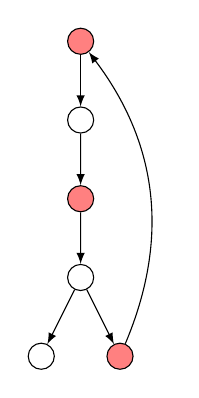
\begin{tikzpicture}[every node/.style={draw,ellipse},edge from parent/.style={draw,-latex},sibling distance=10mm,level distance=10mm]
        \node[fill=red!50,fill on=<2>] (dr) {}
        child {node {}
          child {node[fill=red!50,fill on=<2>] {}
            child {node {}
              child {node {}}
              child {node[fill=red!50,fill on=<2>] (ref) {}}
            }}};
        \draw[-latex, bend right,alt=<2>{red}{black}] (ref) to (dr);
      \end{tikzpicture}
    \end{column}
    \begin{column}{0.75\textwidth}
      \begin{block}{Workflow Before}
        \begin{enumerate}
        \item Compile the formula to a \alert{circuit}
        \item Evaluate to get the answer
        \end{enumerate}
      \end{block}
      \pause
      \begin{block}{Workflow After}
        \begin{enumerate}
        \item Compile the formula to a \alert{graph}
        \item Extract the definitions of functions
        \item Simplify
        \item Supplement with \alert{base cases}
        \item Evaluate to get the answer
        \end{enumerate}
      \end{block}
    \end{column}
  \end{columns}
\end{frame}
% Only Step 1 is fully automated at this point. The other steps are executed by hand.
% Two parts: compilation and inference/evaluation.

\begin{frame}{More Formally\ldots}
  \begin{definition}
    A \alert{first-order deterministic decomposable negation normal form computational graph} (FCG) is a
    \begin{itemize}
    \item directed graph
    \item (which is weakly connected)
    \item with a single source,
    \item labelled vertices,
    \item and ordered outgoing edges.
    \end{itemize}
  \end{definition}
\end{frame}

\begin{frame}{How to Interpret an FCG}
  \begin{columns}
    \begin{column}{0.25\textwidth}
      \centering
      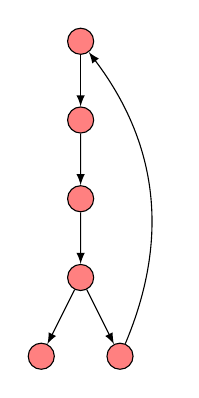
\begin{tikzpicture}[every node/.style={draw,ellipse},edge from parent/.style={draw,-latex},sibling distance=10mm,level distance=10mm]
        \node[fill=red!50,fill on=<2>] (dr) {}
        child {node[fill=red!50,fill on=<3>] {}
                child {node[fill=red!50, fill on=<4>] {}
                  child {node[fill=red!50, fill on=<5>] {}
                    child {node[fill=red!50, fill on=<6>] {}}
                    child {node[fill=red!50, fill on=<7>] (ref) {}}
        }}};
        \draw[-latex, bend right] (ref) to (dr);
      \end{tikzpicture}
    \end{column}
    \begin{column}{0.75\textwidth}
      \begin{align*}
        f(m, n) &= \onslide<3->{\sum_{l=0}^m \binom{m}{l}} \onslide<6->{[l<2]} \onslide<5->{\times} \onslide<7->{f(m-l, n-1)}\\
        \onslide<8>{&= f(m, n-1) + mf(m-1, n-1)}
      \end{align*}
      \onslide<6>{
        \[
          [\phi] =
          \begin{cases}
            1 & \text{if } \phi \\
            0 & \text{if } \neg\phi
          \end{cases}
          \]
      }
    \end{column}
  \end{columns}
\end{frame}

\begin{frame}{Compilation Rules}
  \begin{definition}
    A \alert{(compilation) rule} is a function that takes a \alert{formula} and returns a set of \structure{$(G, L)$} pairs, where
    \begin{itemize}
    \item \structure{$G$} is an FCG,
    \item and \structure{$L$} is a list of formulas.
    \end{itemize}
  \end{definition}
\end{frame}

\begin{frame}{Example Rule: Independence}
  Input formula:
  \begin{gather}
    ({\color{color1} \forall x, y \in \Omega\text{. }x=y}) \land \label{eq:1} \tag{{\color{color1} 1}} \\
    ({\color{color2} \forall x \in \Gamma\text{. }\forall y, z \in \Delta\text{. }P(x, y) \land P(x, z) \Rightarrow y=z}) \land \label{eq:2} \tag{{\color{color2} 2}} \\
    ({\color{color2} \forall w, x \in \Gamma\text{. }\forall y \in \Delta\text{. }P(w, y) \land P(x, y) \Rightarrow w=x}) \label{eq:3} \tag{{\color{color2} 3}}
  \end{gather}
  \pause
  Only one \structure{(G, L)} pair:
  \[
  G = 
  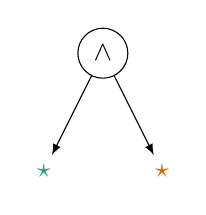
\begin{tikzpicture}[edge from parent/.style={draw,-latex},baseline=(current bounding box.center)]
    \node[draw,circle] {$\land$}
    child {node {\color{color1} $\star$}}
    child {node {\color{color2} $\star$}}
    ;
  \end{tikzpicture},
  \qquad
  L = \langle {\color{color1} \eqref{eq:1}}, {\color{color2} \eqref{eq:2} \land \eqref{eq:3}} \rangle
  \]
  %% Later, both \structure{$G$} and \structure{$L$} are incorporated into a larger \alert{search state}.
\end{frame}
% stars mark edges to nowhere and they are associated with the formulas in L via a certain order

\begin{frame}
  \frametitle<1>{New Rule 1: Generalised Domain Recursion}
  \frametitle<2>{New Rule 2: Constraint Removal}
  \frametitle<3>{New Rule 3: Identifying Possibilities for Recursion}
  \begin{columns}
    \begin{column}{0.15\textwidth}
      \centering
      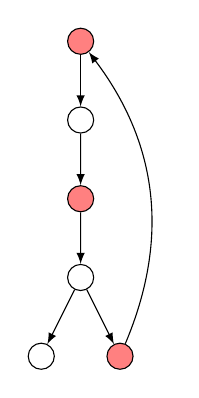
\begin{tikzpicture}[every node/.style={draw,ellipse},edge from parent/.style={draw,-latex},sibling distance=10mm,level distance=10mm]
        \node[fill=red!50, fill on=<1>] (dr) {}
        child {node {}
          child {node[fill=red!50, fill on=<2>] {}
            child {node {}
              child {node {}}
              child {node[fill=red!50, fill on=<3>] (ref) {}}
            }}};
        \draw[-latex, bend right,alt=<3>{red}{black}] (ref) to (dr);
      \end{tikzpicture}
    \end{column}
    \begin{column}{0.85\textwidth}
      \begin{overprint}
        \onslide<1>
          \begin{example}
            Input formula:
            \[
              \forall x \in \Gamma\text{. }\forall y, z \in \Delta\text{. }y \ne z \Rightarrow \neg P(x, y) \lor \neg P(x, z)
            \]
            Output formula (with a new constant \structure{$c \in \Gamma$}):
            \begin{gather*}
              \forall y, z \in \Delta\text{. }y \ne z \Rightarrow \neg P(\alert{c}, y) \lor \neg P(\alert{c}, z) \\
              \begin{multlined}
                \forall x \in \Gamma\text{. }\forall y, z \in \Delta\text{. }\alert{x \ne c} \land y \ne z \Rightarrow \\
                \neg P(x, y) \lor \neg P(x, z)
              \end{multlined}
            \end{gather*}
            %% Output FCG:
            %% \begin{tikzpicture}[edge from parent/.style={draw,-latex}]
            %%   \node[draw,circle] {$\textsc{DR}$}
            %%   child {node {$\star$}}
            %%   ;
            %% \end{tikzpicture}
          \end{example}
        \onslide<2>
          \begin{example}
            Input formula (with a constant \structure{$c \in \Gamma$}):
            \begin{gather*}
              \begin{multlined}
                \forall x \in \alert{\Gamma}\text{. }\forall y, z \in \Delta\text{. }\alert{x \ne c} \land y \ne z \Rightarrow \\
                \neg P(x, y) \lor \neg P(x, z)
              \end{multlined} \\
              \begin{multlined}
                \forall w,x \in \alert{\Gamma}\text{. }\forall y \in \Delta\text{. }\alert{w \ne c} \land \alert{x \ne c} \land w \ne x \Rightarrow \\
                \neg P(w, y) \lor \neg P(x, y)
              \end{multlined}
            \end{gather*}
            Output formula (with a new domain \structure{$\Gamma' \coloneqq \Gamma \setminus \{\, c \,\}$}):
            \begin{gather*}
              \forall x \in \alert{\Gamma'}\text{. }\forall y, z \in \Delta\text{. }y \ne z \Rightarrow \neg P(x, y) \lor \neg P(x, z) \\
              \forall w,x \in \alert{\Gamma'}\text{. }\forall y \in \Delta\text{. }w \ne x \Rightarrow \neg P(w, y) \lor \neg P(x, y)
            \end{gather*}
          \end{example}
        \onslide<3>
          \begin{block}{Goal}
            Check if the input formula is isomorphic (up to domains) to a
            previously encountered formula.
          \end{block}
          \begin{block}{Rough Outline}
            \begin{enumerate}
              \item Consider pairs of `similar' clauses.
              \item Consider bijections between their sets of variables.
              \item Extend each such bijection to a map between sets of domains.
              \item If the bijection makes the clauses equal, and the domain map
                    is compatible with previous domain maps, move on to another
                    pair of clauses.
            \end{enumerate}
          \end{block}
      \end{overprint}
    \end{column}
  \end{columns}
\end{frame}
% We're still creating a vertex in a graph with one outgoing edge.

%% \begin{frame}{Compilation as Search}
%%   \begin{definition}
%%     A \alert{(search) state} is a tuple \structure{$(G, C, L)$}, where:
%%     \begin{itemize}
%%     \item \structure{$G$} is an FCG (or \texttt{null}),
%%     \item \structure{$C$} is a compilation cache that maps integers to sets of pairs $(\phi, v)$, where $\phi$ is a formula, and $v$ is a vertex of $G$ (which is used to identify opportunities for recursion),
%%     \item and \structure{$L$} is a list of formulas (that are yet to be compiled). (Note that the order is crucial!)
%%     \end{itemize}
%%   \end{definition}
%%   The search algorithm combines greedy and breadth-first search:
%% \end{frame}

\begin{frame}{Resulting Improvements to Counting Functions}
  Let \structure{$\Gamma$} and \structure{$\Delta$} be two sets with
  cardinalities \structure{$|\Gamma| = m$} and \structure{$|\Delta| = n$}.

  Our new rules enable \textsc{ForcLift} to efficiently count
  \structure{$\Gamma \to \Delta$} functions such as:
  \begin{itemize}
    \item injections in \structure{$\Theta(mn)$} time
          \begin{itemize}
            \item best: \structure{$\Theta(m)$}
          \end{itemize}
    \item partial injections in \structure{$\Theta(mn)$} time
          \begin{itemize}
            \item best: \structure{$\Theta({\min\{\, m, n \,\}}^2)$}
          \end{itemize}
          \item bijections in \structure{$\Theta(m)$} time
          \begin{itemize}
            \item \alert{optimal!}
          \end{itemize}
  \end{itemize}
\end{frame}
% TODO: mention Crane
% TODO: mention that everything used to be unliftable (by any algorithm with a publicly available implementation)

{ % all template changes are local to this group.
    \setbeamertemplate{navigation symbols}{}
    \begin{frame}<article:0>[plain]
        \begin{tikzpicture}[remember picture,overlay]
            \node[at=(current page.center)] {
                
\includegraphics[keepaspectratio, height=\paperheight]{zoom.jpg}
            };
        \end{tikzpicture}
     \end{frame}
}

\begin{frame}{Summary \& Future Work}
  \begin{block}{Summary}
    The circuits hitherto used for FOMC become more powerful with:
    \begin{itemize}
    \item cycles,
    \item generalised domain recursion,
    \item and some more new compilation rules that support domain recursion.
    \end{itemize}
  \end{block}
  \begin{block}{Future Work}
    \begin{itemize}
    \item Automate:
      \begin{itemize}
      \item extracting and simplifying the definitions of functions,
      \item finding all base cases.
      \end{itemize}
    \item Open questions:
      \begin{itemize}
      \item What kind of \alert{sequences} are computable in this way?
      \item Would using a \alert{different logic} extend the capabilities of FOMC further?
      \end{itemize}
    \end{itemize}
  \end{block}
\end{frame}

\end{document}
